\chapter{Proposed System}
\label{Ch_Chapter3}


We have used two methods for ranking document. One is term frequency and another is cosine similarity.

\section{Creating Document Vector}
The process of creating document vector is given below.

\subsection{Term Frequency}

A term that appears many times within a document is likely to be more important than a term that appears only once.\\
D1: {\unicodefont আমি  বাংলাদেশকে ভালবাসি । বাংলাদেশ নদীমাতৃক দেশ।}  \\ 
D2: {\unicodefont আমি বাংলাদেশের নাগরিক । কিন্তু বাংলাদেশের সকল  নাগরিক তাদের মোলিক অধিকার পায় না।} \\
D3: {\unicodefont বাংলাদেশ উন্নয়নশীল দেশ। এখনো উন্নয়নের দিক থেকে পিছিয়ে আছে বাংলাদেশ । } \\

After performing the term frequency calculation we get the table \ref{tab:tab1}. Which is showing the value each word each document.

\begin{table*}[htp]	
\centering

  \caption{Parameters of datasets }
\vspace{0.5cm}
\begin{tabular}{|c|c|c|c|} 
\hline

\textbf{Term} &\textbf{Doc1} 	 & \textbf{Doc2} &\textbf{Doc3}   \\ \hline
{\unicodefont আমি} 		& 1 & 1 &	   \\ \hline
{\unicodefont বাংলাদেশ}	& 2 & 2 & 2   \\ \hline
{\unicodefont ভালবাসি }	& 1 &  &   \\ \hline
{\unicodefont উন্নয়নশীল } 	&  &  &   \\ \hline
{\unicodefont দেশ } 	&  &  & 1  \\ \hline
{\unicodefont নদীমাতৃক }  & 1 &  &   \\ \hline
{\unicodefont কিন্তু}	&  & 2 &   \\ \hline
{\unicodefont সকল}সকল	&  & 1 &   \\ \hline
{\unicodefont মোলিক}	&  & 1 &   \\ \hline
{\unicodefont অধিকার}	&  & 1 &   \\ \hline
{\unicodefont পায়}	&  & 1 &   \\ \hline
{\unicodefont এখনো}	&  &  & 1  \\ \hline
{\unicodefont দিক}  &  &  & 1 \\ \hline
{\unicodefont থেকে} &  &  & 1 \\ \hline
{\unicodefont পিছিয়ে}&  &  & 1 \\ \hline
{\unicodefont আছে}&  &  & 1 \\ \hline
{\unicodefont নাগরিক}&  & 2 &  \\ \hline
{\unicodefont না} &  & 1 &  \\ \hline
{\unicodefont তাদের}&  & 1 &  \\ \hline

\end{tabular}
\label{tab:tab1}
\end{table*}



\subsection{Stop Word Removing}
Documents contain words that do not add information but are necessary for syntactical formation,such as words like {\unicodefont এবং , অথবা , কিন্তু } etc. Since these words are less useful and less informative,  they introduce  noise into the document representation. In order to get rid of these kind of words, a stop word removal step is used.  Stop word removal is done using predefined, human-made list of words. Since a predefined list is used, this approach is language dependent. Instead of using these kinds of lists, a frequency threshold can be used. If a word is seen more\/less frequently than predefined threshold, that word can be considered as stop word. But decision of threshold is another issue to be considered.

\subsection{Stemming}

In a document a word can be seen in different formats, such as plural vs. singular, present vs. past tense, etc. Most of the time these words have the same meaning and treating them differently is unnecessary. In order to use these words as the same token(concept), stemmers are used.
Stremmers are tools that reduce the orginal word forms into roots(stems) of these words. Stemmers are necessary to represent different forms in a single format and to reduce memory usage for storing the words. Also, smaller list of words make it easir to perform calculations. As a result of performing stemming,document representation is less noisy and more dense. The efficiency of a stemmer is important while performing further calculations. In Figure \ref{Figure:stemm} ,we can see the full process of ranking.

Sometimes stemmers can do over-stemming such that two words are given the same stem,while it should not be. For example, the words {\unicodefont “বাংলাদেশের”} and {\unicodefont “বাংলাদেশকে”} are two different words, which should not be stemmed into the same root. But stemmers can find out their root as {\unicodefont “বাংলাদেশ”}. Another steamming problem is related to under stemming such that two words should have been stemmed into the same word, but have not been. for example, {\unicodefont “হাসি”} and {\unicodefont ‘হাসানো’} can be found as two different stems,instead of one.



\subsection{Weighting Term}

Then find weight in a document for each term using the equation \ref{eq:eq1}

\begin{equation}
Weight++=postings[term][doc]*IDF
\label{eq:eq1}
\end{equation}

%\(Weight++=postings[term][doc]*IDF\)

Then assigning document IDS we keep them into database as vector after doing following steps which is shown in Figure \ref{Figure:indexing}.

\subsubsection{Inverse Document Frequency(IDF)}

A term that occurs in a few documents is likely to be a better discriminator than a term that appears in most or all documents.

Then assigning document IDS we keep them into database as vector after doing these steps.


\begin{figure*}[htp]
	\centering
		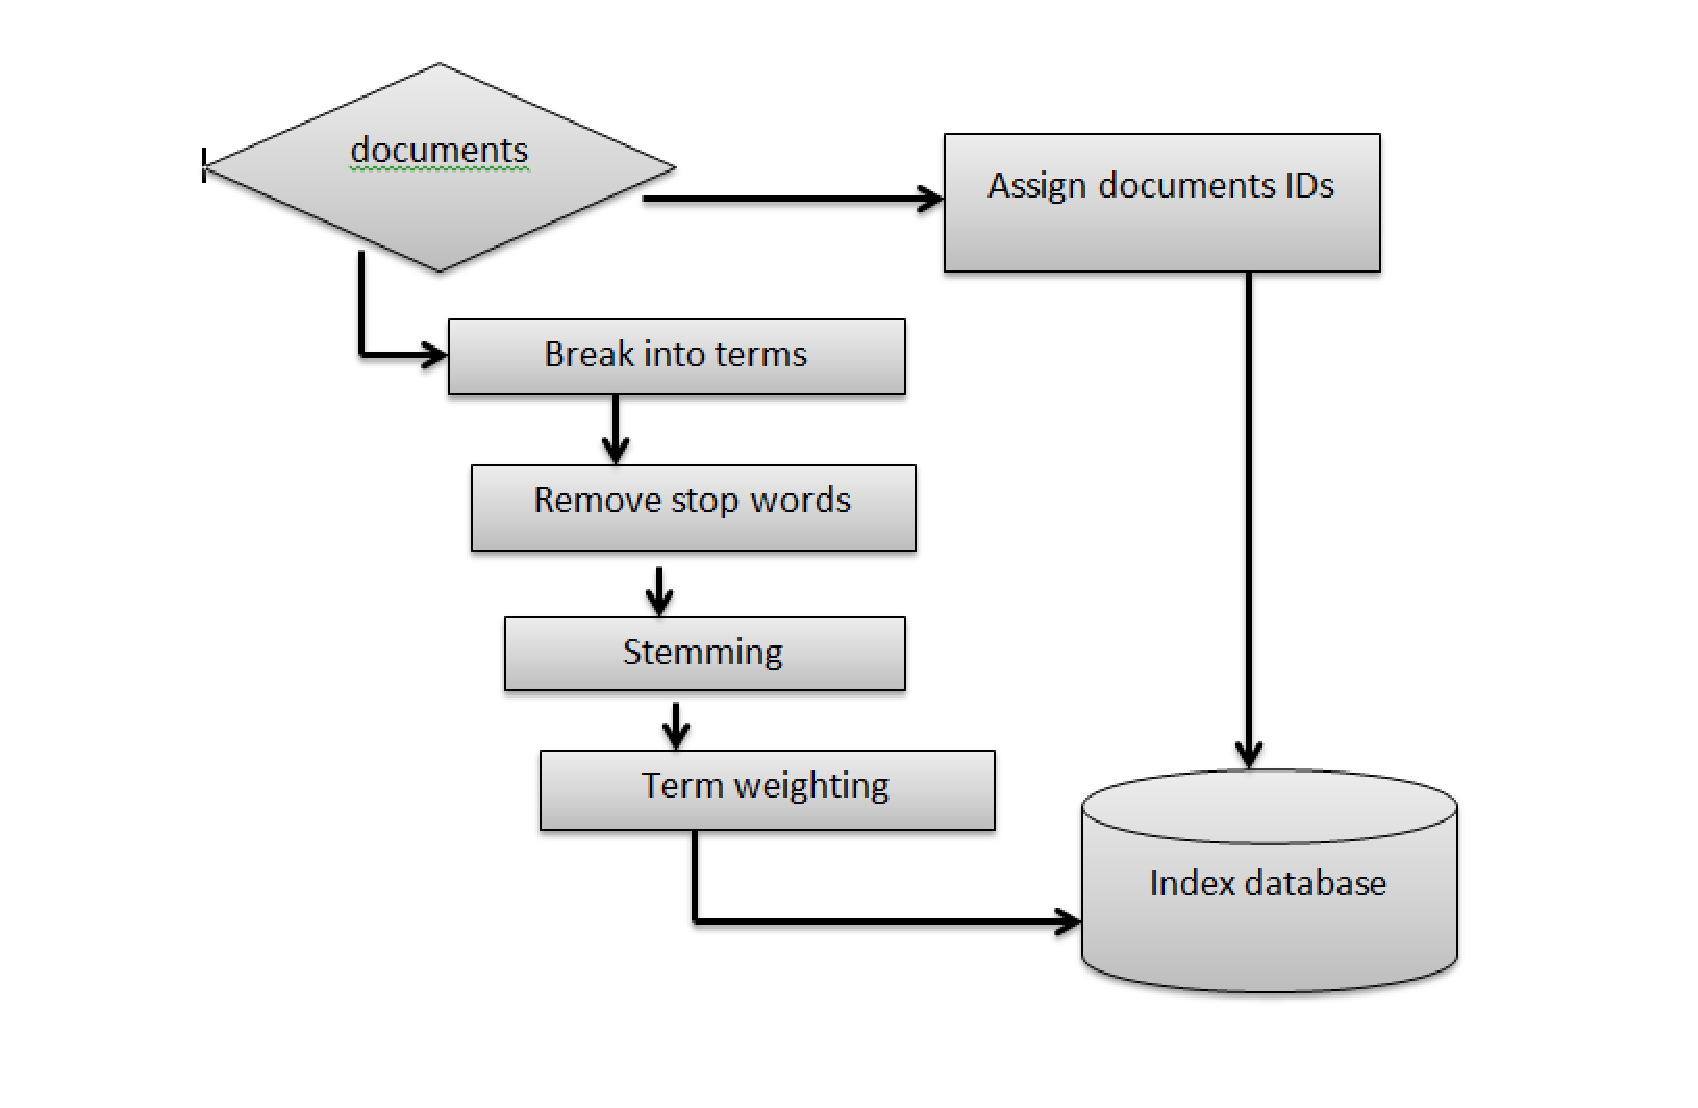
\includegraphics[width=.65\textwidth]{figure/two.eps}
	\caption{Indexing Document Ids \& keep it in a vector.}
	\label{Figure:indexing}
\end{figure*}


\section{Preprocessing of Taking Query}

For taking search query the preprocessing steps have to be done. After taking query step by step process has been done . And then match query with relevent documents. The preprocessing steps are showing in the figure \ref{Figure:inquery} below.


\begin{figure*}[htp]
	\centering
		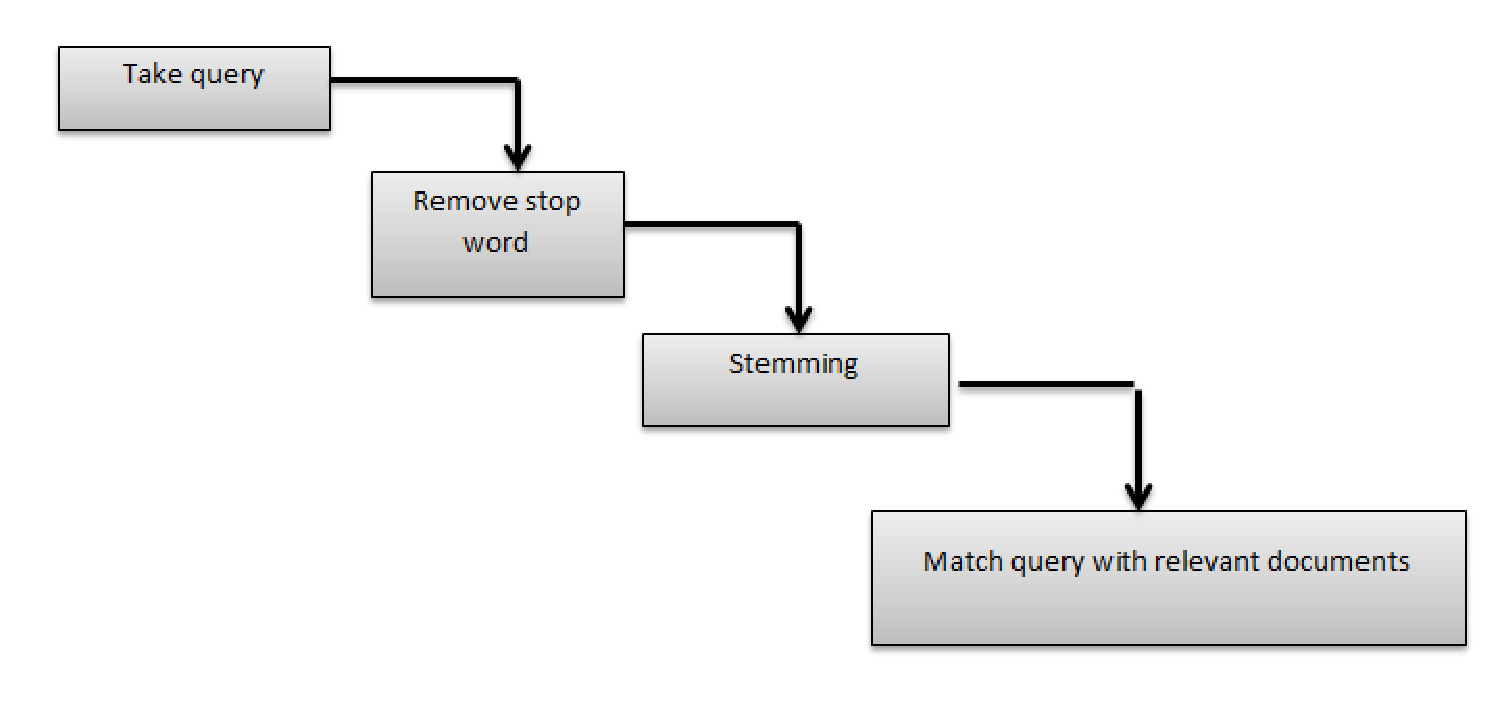
\includegraphics[width=.65\textwidth]{figure/three.eps}
	\caption{Pre processing of Input query}
	\label{Figure:inquery}
\end{figure*}


\subsection{Removal of Stop Word}

The less importance word should be removed from query. Sometimes input query contain words that do not add information, such type words {\unicodefont ‘এবং’ , ‘অথবা’ , ‘কিন্তু ’} etc should remove from document.

\subsection{Stemming}

Finding root words from other similar words which have the same meaning and treating them differently is unnecessary. Figure \ref{Figure:stemm} showing the process.

\begin{figure*}[htp]
	\centering
		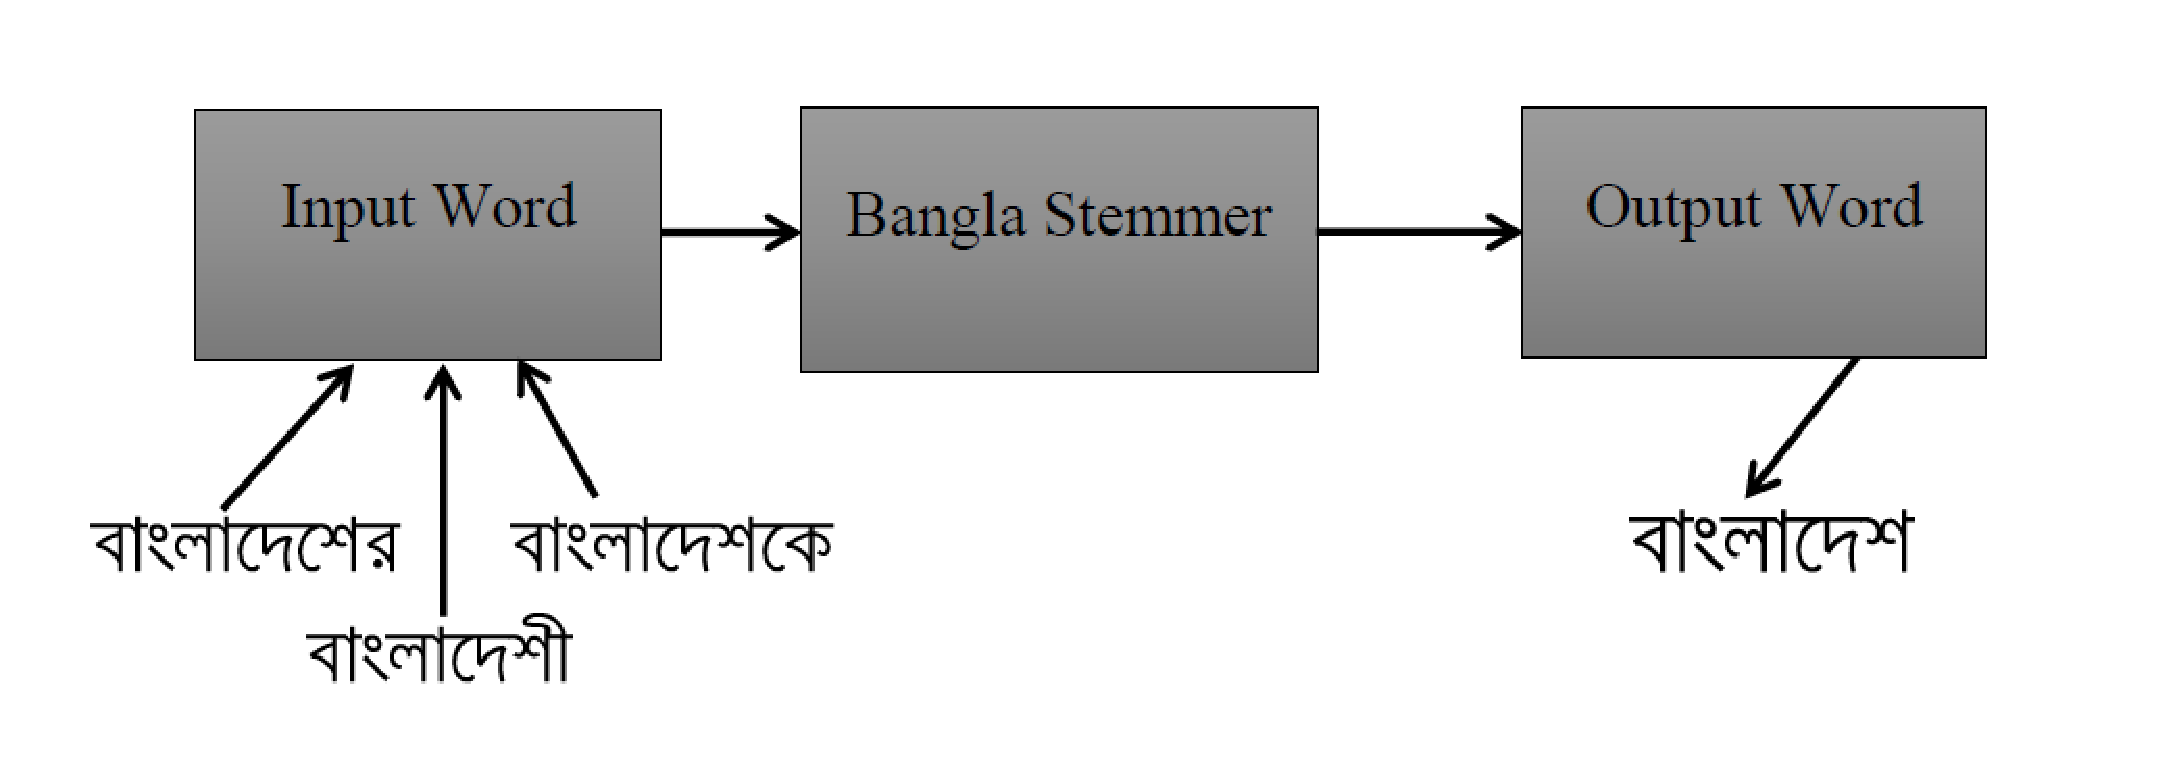
\includegraphics[width=.65\textwidth]{figure/four.eps}
	\caption{Stemming processing}
	\label{Figure:stemm}
\end{figure*}


\section{Cosine Similarity}

The query matches with relevent documents. If exists, find out the relevent documents and give them a scores using query term’s IDF multiplying with weight. Then sort the values and rank the documents.

Example:
There are three documents.\\
	D1: {\unicodefont আমি  বাংলাদেশকে ভালবাসি । বাংলাদেশ নদীমাতৃক দেশ।} \\
	D2: {\unicodefont আমি বাংলাদেশের নাগরিক । কিন্তু বাংলাদেশের সকল  নাগরিক তাদের মোলিক অধিকার পায় না। }\\
	D3: {\unicodefont বাংলাদেশ উন্নয়নশীল দেশ। এখনো উন্নয়নের দিক থেকে পিছিয়ে আছে বাংলাদেশ ।  }\\
	
	%{\unicodefont বাংলাদেশের নাগরিক হিসেবে বাংলাদেশের উন্নতি চাই।}
Input Query: {\unicodefont বাংলাদেশের নাগরিক হিসেবে বাংলাদেশের উন্নতি চাই।}\\

\(Cosine(document , query)  = (document . query) / |document vt | |query vt|\)\\


Now in table \ref{tab:Scoring} we can see the scores after doing the all process.

\begin{table*}[htp]	
\centering

\caption{Scoring Each Document  }
\vspace{0.5cm}
\begin{tabular}{|c|c|c|} 
\hline

	\textbf{Document Id }& \textbf{Documents} & \textbf{Scores} \\ \hline
 1 & D1 &	0.145   \\ \hline
 2 & D2 & 0.543   \\ \hline
 3 & D3  &0.345   \\ \hline


\end{tabular}
\label{tab:Scoring}
\end{table*}

After sorting scores, we get the ranked documents and we can see that in table \ref{tab:Rank}.


\begin{table*}[htp]	
\centering
\caption{Rank Documents  }
\vspace{0.5cm}
\begin{tabular}{|c|c|c|} 
\hline

\textbf{Document Id}  & \textbf{Documents} & \textbf{Scores} \\ \hline
 2 & D2 &	0.543   \\ \hline
 3 & D3 & 0.345   \\ \hline
 1 & D1 &0.145  \\ \hline


\end{tabular}
\label{tab:Rank}
\end{table*}


\section{Main Approaches}

When the preprocessing is completed, then our main process focuses on the analysis of the processed output by our own developed tools for Bangla document ranking. Our main approach are includes to generating term frequency vector, assigning cosine similarity to the corresponding document are known as document scoring. Then sorting the scores, we rank the documents. In figure \ref{Figure:graphical} shows the overall graphical view of our proposed system.

\begin{figure*}[htp]
	\centering
		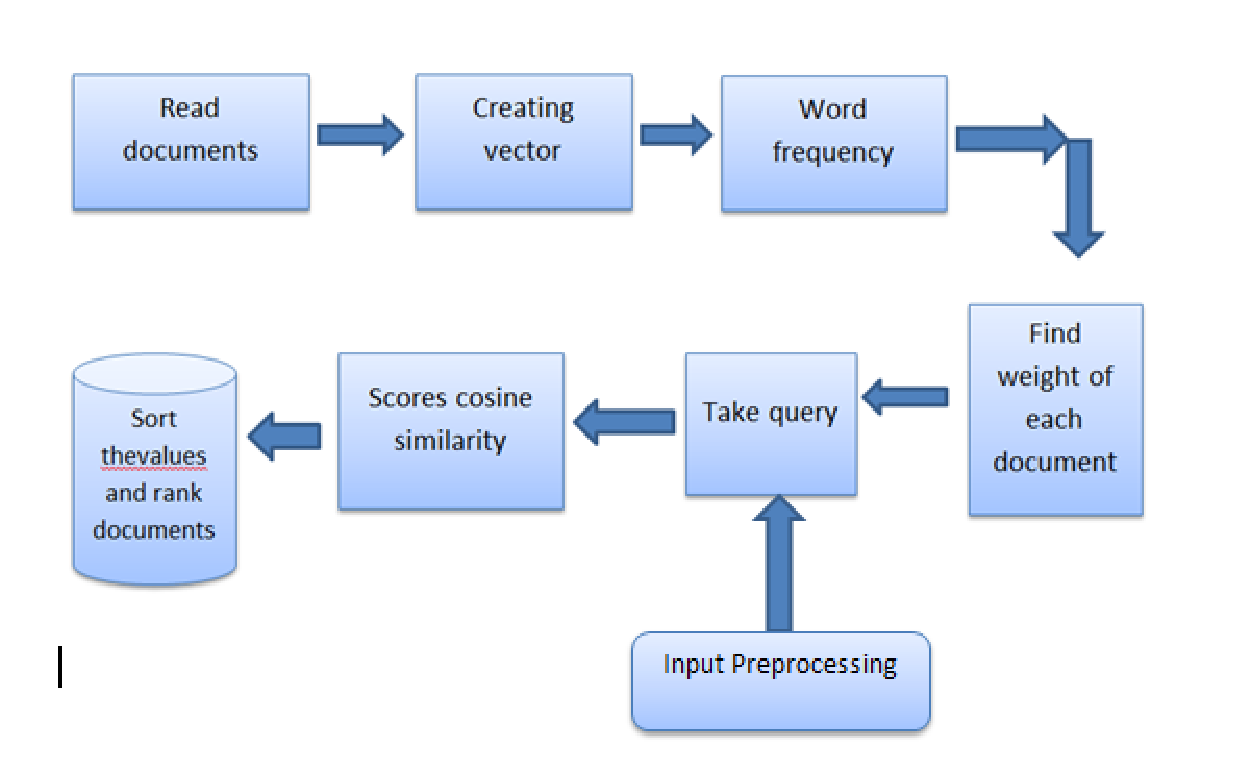
\includegraphics[width=.65\textwidth]{figure/five.eps}
	\caption{Overall graphical view of our proposed system}
	\label{Figure:graphical}
\end{figure*}

